\documentclass[14pt,a4paper]{scrartcl}
%too many packeges
\usepackage[utf8]{inputenc}
\usepackage[english]{babel}
\usepackage{indentfirst}
\usepackage{misccorr}
\usepackage{apacite}
\usepackage{graphicx}
\usepackage[section]{placeins}
\usepackage{float}
\usepackage{tabularx}
\usepackage{color}
\usepackage{fancyhdr}
\usepackage{times}
\usepackage{gensymb}
\usepackage{verbatim}
\usepackage{mathtools}
\usepackage{titlesec}
\usepackage{url}
\usepackage[T1]{fontenc} 
\usepackage{sectsty}
\usepackage{natbib}
\usepackage{makecell}
\usepackage{dsfont}
\usepackage[labelsep=period]{caption}
\usepackage{subcaption}
\usepackage{setspace}
\usepackage{titletoc}
\usepackage{mathrsfs}
\usepackage{circuitikz}
\usepackage{tcolorbox}
\usepackage{lipsum}
\usepackage{mathptmx}
\usepackage{caption} % hypcap is true by default so [hypcap=true] is optional in \usepackage[hypcap=true]{caption}
\usepackage[nottoc,notlot,notlof]{tocbibind}
\definecolor{mygray}{gray}{0.4}
\usepackage[top=2.5cm,bottom=2.5cm,right=2.5cm,left=2.5cm,bindingoffset=0cm]{geometry}
\usepackage[colorlinks=true, a4paper=true, pdfstartview=FitV,
linkcolor=black, citecolor=mygray, urlcolor=black]{hyperref}

\DeclareMathOperator*{\argmax}{arg\,max}

%formating routine
\titleformat{\subsection}[block]{\bfseries{\hspace{2em}}}{\thesubsection}{1em}{}
\titleformat{\subsubsection}[block]{\bfseries{\hspace{3em}}}{\thesubsubsection}{1cm}{}
\newcommand{\sectionbreak}{\pagebreak}
\sectionfont{\centering}
\renewcommand{\baselinestretch}{1.5}
\captionsetup{compatibility=false}
\setlength{\parindent}{0.5in}
\setlength{\parskip}{6pt}
\graphicspath{ {images/} }
\linespread{1.25}
\pdfcompresslevel=9

%Macros for numeration
\makeatletter
\renewcommand{\@seccntformat}[1]{%
  \ifcsname prefix@#1\endcsname
    \csname prefix@#1\endcsname
  \else
    \csname the#1\endcsname\quad
  \fi}
\newcommand\prefix@section{Chapter \thesection. }
\makeatother
%Hack for prefixes in toc
\titlecontents{section}[3.5em]{\medskip\bfseries}
{\contentslabel[\color{black}Chapter \thecontentslabel]{4.5em}\enspace}
{\hskip-3em}
{\titlerule*[1.2pc]{.}\contentspage}

\newcommand{\norm}[1]{\left\lVert#1\right\rVert}
\begin{document}

	\begin{titlepage}
		  \begin{center}
		    \large
		    \textbf{The Government of the Russian Federation}
		    
		    \textbf{Federal State Autonomous Educational Institution\\of Higher Professional Education}
		    \vspace{0.25cm}
		    
		   \textbf{National Research University – Higher School of Economics}
		   \vspace{0.25cm}

		   	Faculty of Social Sciences
		    \\School of Psychology\\[1cm]
		    
		    \textbf{Undergraduate Thesis}
		    \\[0.5cm]
		    \textbf{\guillemotleft Neurophysiological Correlates Of Efficient Learning In The Neurofeedback Paradigm \guillemotright}
		    \vfill
		     
			\end{center}

	\newlength{\ML}
	\hfill\begin{minipage}{0.4\textwidth}
	  \textbf{Student group BPS-143}\\[0.3cm]
	  \underline{Minkov V.\,A.} \\
	  \scriptsize{Last name, First name, Middle name}\\\\
	  \large
	  \underline{\hspace{7cm}}
	  \scriptsize{Signature}\\
			\end{minipage}%


	\hfill\begin{minipage}{0.4\textwidth}
	  \textbf{Scientific adviser}\\[0.3cm]
	  \underline{Professor\, PhD} \\
	  \scriptsize{Position, Academic degree}\\\\
	  \large
	  \underline{Ossadtchi A.\,E.} \\
	  \scriptsize{Last, F. M/O.}\\\\
	  \underline{\hspace{7cm}}
	  \scriptsize{Signature}\\
			\end{minipage}

	\hfill\begin{minipage}{0.4\textwidth}
		\textbf{Consultant}\\[0.3cm]
		\underline{Smetanin N.\,M.} \\
		\scriptsize{Last, F. M/O.}\\\\
		\underline{\hspace{7cm}}
		\scriptsize{Signature}\\
			\end{minipage}

	    \vfill
	    \vfill
	    \vfill  

		\begin{center}
		\vfill
		  Moscow, 2018
		\end{center}
	\end{titlepage}


\newpage
\tableofcontents
%Formating routine again
\fancyhf{} 
\renewcommand{\headrulewidth}{0pt} 
\footskip = 30pt
\fancyfoot[R]{\thepage} 
\pagestyle{fancy}
\fancypagestyle{plain}{
  \fancyhf{}
  \renewcommand{\headrulewidth}{0pt}
  \fancyhf[lef,rof]{\thepage}
}
\addtocontents{toc}{\protect\thispagestyle{empty}}

%All party here
\newpage
\section{Introduction}
\label{sec:Introduction}

Operant conditioning is a special way of forming reflexes (involuntary movements in response to a stimulus), that implies reinforcing a reaction that occurs spontaneously, that is, due to the consequences: reinforcement or punishment. The concept of operant conditioning was introduced by Burrhus Frederic Skinner \cite{Skinner1971a,Skinner1971,Skinner1950,Jones1939}, although a similar phenomenon was first extensively studied by \cite{Thorndike1898} a few decades earlier. There is a number of studies on brain activation evoked by the operant conditioning. A group of brain structures responsible for the operant conditioning is widely recognized as part of the rewarding system – neural network responsible for emotions, incentive salience and learning \cite{Schultz2015}. 

Neurofeedback is a procedure that involves real-time displays of brain activity to reward a subject \cite{Kamiya2011}. According to definition, it appears to be a reinforcement learning process and its efficiency critically depends on the extent to which the feedback signal is matched to the particular subject. Feedback signal latency, color, shape, pitch, timbre, etc. are the ergonomic parameters that may potentially strongly affect the efficiency of learning and the intensity of plastic changes – brain’s ability to change throughout life. Finding the proper ergonomic settings for each particular patient has a potential to boost the efficacy of the neurofeedback therapy and to further prove its usefulness in treating various neurological diseases.
\newpage
\section{Hypothesis}
\label{sec:Hypothesis}

\subsection{Reinforcement Learning}
\label{sec:Hypothesis:Reinforcement Learning}

\subsubsection{Definition}
\label{sec:Hypothesis:Learning Process:Definition}

\textit{Reinforcement learning (RL)} is learning process that involves interaction with the environment. Training occurs due to the RL agent's evaluation of their actions and does not imply the receipt of the external instructions. The agent is in a choice situation, which must be resolved by trial and error. A reinforcement signal is a reward that codes the level of success of resolution of a task. The agent seeks to learn how to maximize reward over time. 

Nowadays reinforcement learning is considered in different fields, including machine learning and neurophysiology, and it is based on the theories of classical and instrumental conditioning. Therefore, it is necessary to narrow the field of application of this term. In this study, it will be used as a synonym for operant conditioning. 

\subsubsection{Historical Background}
\label{sec:Hypothesis:Learning Process:Historical Background}

Experiments of \textit{Burrhus Frederic Skinner (1904 - 1990)} with the pigeons are widely known \cite{Skinner1948,Lanza1982,Epstein1981}. Pigeons did not create a great culture, there is no Schopenhauer or Goethe among pigeons. Being trapped in a metal cage with a mechanism that gives out a portion of the feed when the button is pressed, a pigeons will not be able to think through the algorithm of its actions to obtain <<reinforcements>>. However, after making a sequence of random movements, it can accidentally press the button. In this case, the probability that the sequence of the same actions in the future will repeat increases. This phenomenon is called the operant conditioning. Some random actions of the pigeon are reinforced, due to which new reflexes are developed. The term was formulated by different researchers throughout the twentieth and even the nineteenth century. Among them \textit{Ivan Mikhaylovich Sechenov (1829 - 1905)}, Russian physiologist; \textit{Edward Lee Thorndike (1874 - 1949)}, an American psychologis, pioneer of <<the law of effect>>; \textit{Alexei Alexeyevich Ukhtomsky (1875 – 1942)}, Russian and Soviet physiologist; \textit{Jerzy Konorski (1903 - 1973)} and \textit{Stefan Miller (1903 - 1942)}, Polish neurophysiologist. Although it is commonly believed that Skinner's definition was the most accurate definition and it was backed up by the empirical evidence. 

We must admit that the Skinner's system of learning is very detailed. Skinner considered himself a follower of Pavlov. \textit{<<Twenty-five Years of Objective Study of the Higher Nervous Activity of Animals>>}, one of Pavloves's main works, was his reference book \cite{Skinner1971}. Therefore, he began to distinguish two types of behavior, operant and respondent, and even developed a more detailed classification of them. 

Skinner criticized Thorndike in his works for the complexity of the determinization of the processes he studied. Edward Chace Tolman (1886 – 1959), an American psychologist, sharpened this problem, pointing out that during great time intervals various complex constructs might take place \cite{Tolman1948}. Therefore, it may seem that Skinner made the mistake of simply repeating Thorndike's research without paying attention to Tolman. However, there is a very important difference between Skinner and his predecessors.

On the one hand, Skinner refuses from mental representations of needs. Following Pavlov and the behaviourists of the American school, Skinner proposes to abandon the analysis of mental representations in favor of studying the observed behavior and its consequences. On the other hand, Skinner established experimental conditions in which behavior can not be influenced by external factors in his experiments with animals. Thus, within the framework of the American tradition of behavioral research, Skinner was in fact an extremely important figure, because he opened the way for studying psychological phenomena from a physiological and experimental point of view, explaining such a complex process as learning without resorting to additional mechanisms such as cognitive constructs. Thanks to Skinner apparently biological psychology has become possible in the USA. It is interesting to study, thanks to whom a similar situation has developed in Russia, but this is another research, rather, a historical one. In our study, Skinner's position, behavioural one, is fundamentally important, because we would like to record the most low-level processes related to conditioning.

\subsubsection{Modern Concepts Of The Learning Process}
\label{sec:Hypothesis:Learning Process:Modern Concepts Of The Learning Process}

% \begin{figure}[H]
% \centering
% 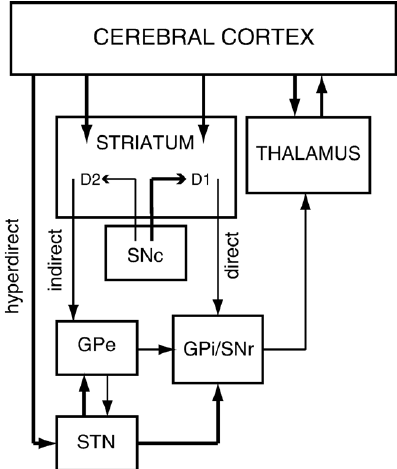
\includegraphics[width=0.7\linewidth]{Schematic-diagram-of-the-basal-ganglia-thalamocortical-circuits-Excitatory.png}
% \caption{Model of cortico-basal ganglia-thalamo-cortical loop. Anatomical studies seem to link conditioning processes with this system. From \label{fig:Schematic-diagram-of-the-basal-ganglia-thalamocortical-circuits-Excitatory.png}
% \end{figure}

On the one hand, in the field of behavioral neuroscience, considering the fact that many animals live without a well developed neocortex, like reptiles and anamniotes, many studies seem to focus on the role of basal ganglia (a group of subcortical structures) in the process of learning. For example, it was suggested that the amygdala, an important part of basal ganglia, plays a chemosensory role and also takes part in the formation of emotions, since the amygdala actually participates in mediating emotional reactions to chemical signals \cite{Martinez-Garcia2010}. Anatomical studies have shown that the amygdala is connected to the olfactory bulb, which affects the perception of sexual pheromones. Although, such results might stress the role of basal ganglia in the process of learning, they do not seem to be absolutely relevant to humans, as they have a more developed neocortex that shares some functions of basal ganglia in the animal brain.

% \begin{figure}[H]
% \centering
% 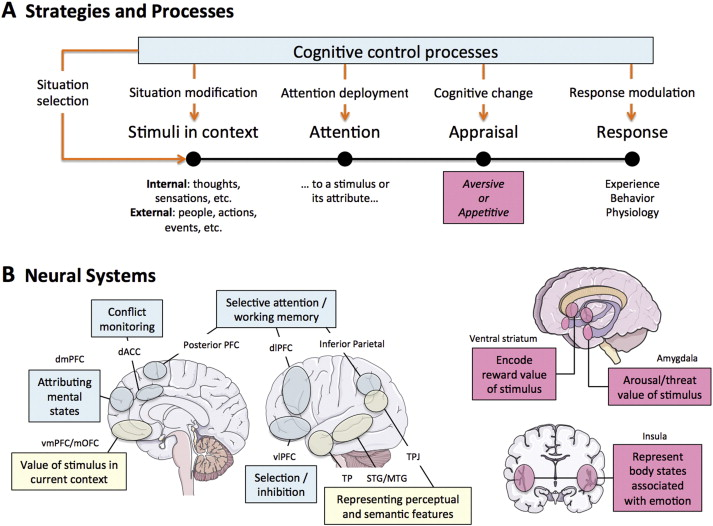
\includegraphics[width=0.7\linewidth]{cc}
% \caption{Brief cognitive control description. Cognitive studies seem to link the conditioning process to this system. From \cite{Val-Laillet2015}\label{fig:cc}
% \end{figure}

On the other hand, in the field of cognitive neuroscience, the term «cognitive control» has recently been developed, which includes the function of reinforcement learning \cite{Cockburn2011,Val-Laillet2015}. Cognitive control is a collective term describing interrelated processes linked to flexible, purposeful behavior. For example, \cite{Ridderinkhof2004} in their review of primate and human studies, along with a meta-analysis of the human functional neuroimaging literature has shown that the medial frontal cortex, or rather its part, anterior cingulate cortex, is believed to be involved in such processes as monitoring the need for increasing cognitive control; behavior correction by sending signals to other cortical structures. Comparing this work to the previous one, we may say that the researchers stress the role of neocortex forgetting about the basal ganglia, which might be insufficient for our research.

As we may see from the works we’ve covered, although the «reward system» and cognitive control are terms that represent different concepts, they are interrelated, because similar structures correlate with their activation, namely the anterior cingulate cortex; different researchers attribute similar functions to both systems; and the reward system, and cognitive control are associated with targeted behavior, and therefore with operant conditioning. Using an integrative approach, suggested by Cockburn and Frank \cite{Cockburn2011}, taking under the consideration both the role of basal ganglia and the role of neocortex, may help to interpret data received from human reward system. For instance, cognitive control theory of beta-wave part may be applied to our research as it attracts our scientific interest.

Why should we integrate these two concepts? The fact is that studies for cognitive control have rich data linking the learning processes with brain rhythms and electroencephalography.

First, it was established that the medial prefrontal cortex generates a high-power theta waves in the conflict of motor tasks. The study by Luu and Tucker \cite{Luu2001} has shown that the mean and lateral oscillations are present for both correct and erroneous answers. When an error occurs, the oscillation of the midline is typed strongly. The initial analysis localizes the oscillation of the midline to the central frontal cortex and lateral oscillations to the sensorimotor cortex. Unfortunately, the study is focused on theta waves and there is no opposition to erroneous answers given. As we have already said, we would prefer to be able to monitor both correct and erroneous answers.

Secondly, the most popular theory of frontal beta waves suggests that the power of this rhythm increases in case of effective performance of the task, and supports the current motor and cognitive state with the help of top-down control. Engel and Fries \cite{Engel2010} have shown that beta activity indicates whether the current sensorimotor or cognitive state is supported. However, just as in the previous study, this one tends to register correct answers only, not paying attention to the wrong ones.

Our main concern was that such complex functions as, for example, the processing of the answer, may not reach the threshold of awareness, but will still have physiological correlates, which Gaal and Lamme have shown in one of their studies \cite{VanGaal2012}.

\subsection{Neuroelectricity}
\label{sec:Hypothesis:Bioelectricity}

\subsubsection{Definition}
\label{sec:Hypothesis:Bioelectricity:Definition}

\textit{Neuroelectricity} is a type of bioelectricity, relating to the electrical phenomena (as potentials or signals) generated by the nervous system. \textit{Bioelectricity} is a general term that is used to encompass electrical potentials and currents occurring within or produced by living organisms. Conversion of chemical energy to electrical energy causes bioelectrical processes. The main difference between electricity in biological and artificial systems is that bioelectrical current is a flow of ions, while standard electricity is a movement of electrons. Since we conducted a neurophysiological study, in this section we will focus on the role of neuroelectricity.

\subsubsection{Historical Background}
\label{sec:Hypothesis:Bioelectricity:Historical Background}

\begin{figure}[H]
\centering
\begin{minipage}{.5\textwidth}
  \centering
  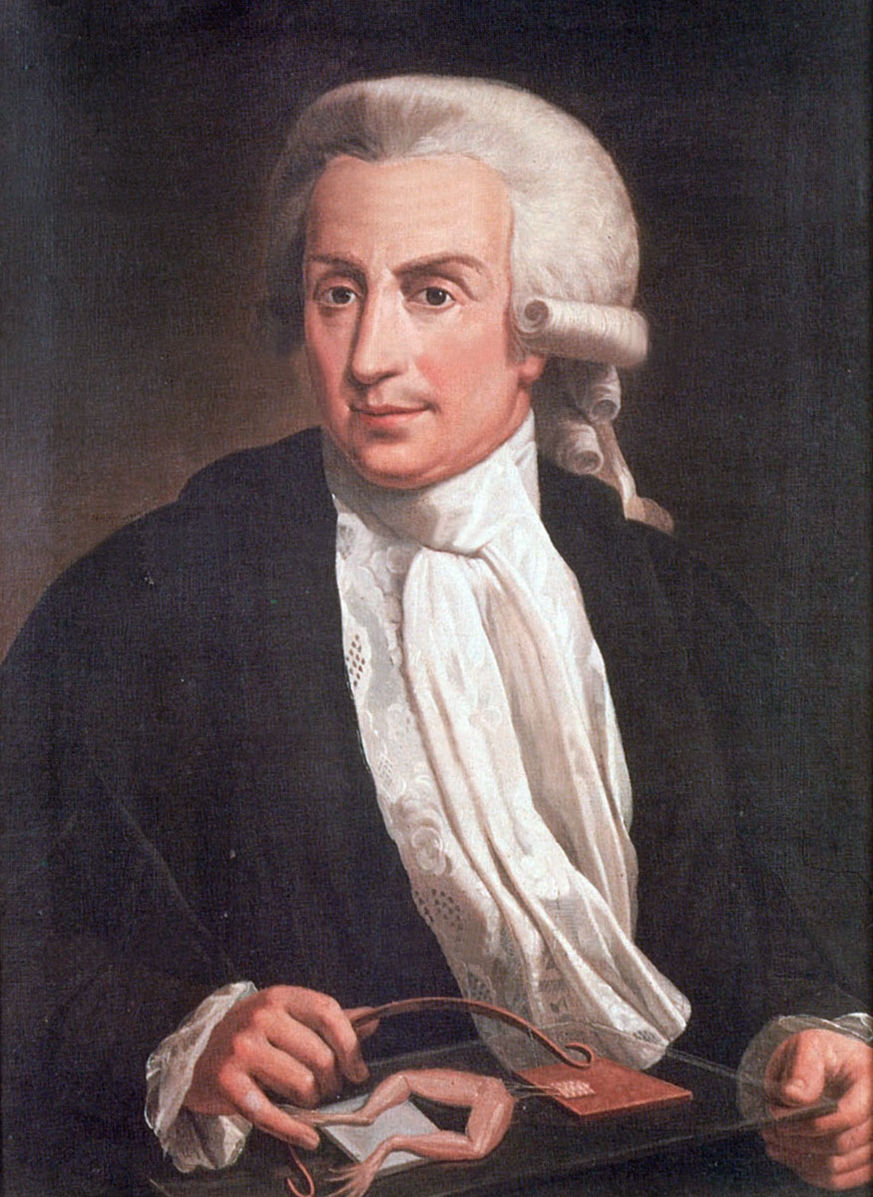
\includegraphics[width=0.5\linewidth]{Galvani}
  \captionof{figure}{Luigi Galvani}\label{fig:Galvani}
\end{minipage}%
\begin{minipage}{.5\textwidth}
  \centering
  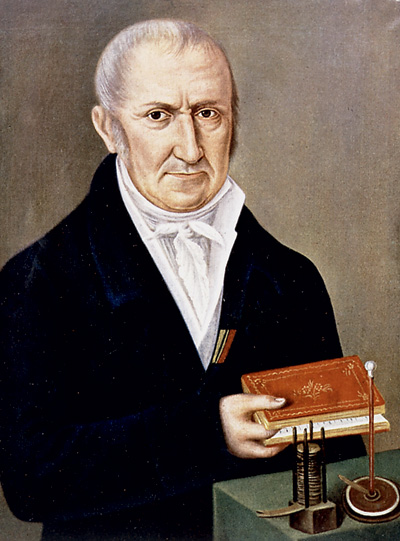
\includegraphics[width=0.5\linewidth]{Volta}
  \captionof{figure}{Alessandro Volta}\label{fig:Volta}
\end{minipage}
\end{figure}

The study of bioelectricity began in 18th century by the physicist \textit{Alessandro Volta} (1745 — 1827) and the physician \textit{Luigi Galvani} (1737 – 1798). Volta created the battery and studied electricity outside of living systems, while Galvani studied electricity in frogs. They both demonstrated that the true explanation of nervous conduction is bioelectricity. However, despite the fact of having common interests, Galvani believed that <<animal electricity>> was fundamentally different from the <<heat electricity>> Volta was studying was studing at the time. We know, that Galvani was wrong, but even nowadays these conflict seems to be reasonable, as manifestation and rules are so different, such as between neuron and galvanic cell, that one might think differently about electricity in artificial and living systems.

\textit{Emil Du Bois-Reymond} was the developer of experimental electrophysiology, the study of the electrical properties of biological cells and tissues. He discovered ways of measuring the tiny electrical currents generated by living tissue. \textit{Julius Bernstein}, a German physiologist, who studied medicine at the University of Berlin with Emil Du Bois-Reymond, hypothesised that nerve and muscle fibers are normally polarized, with positive ions on the outside and negative ions on the inside. According to his theory, the current of living systens results from the reverse of the polarization.

\subsubsection{Electrical Activity of Single Neurons}
\label{sec:Hypothesis:Bioelectricity:Electrical Activity of Single Neurons}

In this section, three types of electrical activity of neurons will be considered: the rest potential (RP), the action potenial, the postsynaptic potential (PSP). All of the above types of potentials occur at a microscopic level. It is necessary to give them a definition to deal with the processes occurring at the macroscopic level: the event related potentials (ERP) and neural oscillation. Both ERP and Neural oscillation are of interest in this study, because they can be registered non-invasively. For example, using EEG.

The resting potential (RP) is a relatively stable potential of the cell membrane of an excitable cell (neuron, myocyte). The presence of a resting potential is the result of the vital activity of a neuron, the joint functioning of all cell organelles. The appearance of the $K^{+}$-channels on the membrane is the sign of neuron maturation. Equilibrium potential is ensured by the operation of the sodium-potassium adenosine triphosphatase protein (sodium–potassium pump), which exchanges in-cell $Na^{+}$ ions for $K^{+}$ ions from the intercellular substance, while expending the energy liberated during the cleavage of the ATP molecule to ADP. An ion gradient results from sodium–potassium pump work \cite{Purves2004}. 

The coming out of $K^{+}$ ions is accompanied by the accumulation of a negative charge inside the cytoplasm. Negative charge gradually slows down the diffusion. After a while, a state of dynamic equilibrium arises, in which the number of $K^{+}$ ions leaving the cell is equal to the number of ions entering one. Therefore, the rest potential is primarily the charge of the membrane of the excited cell, which is provided by the diffusion of potassium ions into the intercellular environment. But there are other ions affecting the RP. Using the Nernst equation, the equilibrium potential of $K^{+}$ and other ions that determine the value of the rest potential can be calculated \cite{Purves2004}.

\begin{equation}
E = E^{0} + {\frac{RT}{nF}}\ln{\frac{X_{out}}{X_{in}}}
\end{equation}

where $E_k$ is the equilibrium potential for the ion $X$; $E_0$ is the standard electrode potential; $R$ is the gas constant; $T$ is the absolute temperature; $F$ is the Faraday number; $n$ is the valency of $X$; $[X_{out}]$ - $[X_{in}]$ - external and internal concentrations of $X$.

One gets an equilibrium potential or transmembrane potential of the resting cell by keeping the negative lead of the voltmeter out of the cell and putting the positive lead inside of the cell $V_{trans} = \phi_{inside} - \phi_{outside}$. Axisal potential is got by keeping the negative lead further from the cell body and the positive lead closer to the cell body $V_{axial} = \phi_{b} - \phi_{a}$.

$Na^{+}$ ions are fundamentally important. The equilibrium potential for potassium ions in mammals is about $-90 mV$. But due to the normal leakage current of $Na^{+}$, the RP is shifted closer to zero and is approximately $-70 mV$. There are constantly open $Na^{+}$ channels on the membrane of the neuron. The excess of sodium ions in the intercellular environment and the negative charge of the cytoplasm lead to entry of sodium ions into the cell and provide this displacement. The larger offset is limited by the small number of permanently open channel and constant work of sodium–potassium pump \cite{Purves2004}. 

There are two main types of change in the resting potential arising on neuronal membranes: action potential (AP) and postsynaptic potential (PSP). AP is the response of the nerve cell to stimulation; a discrete depolarization waves propagating from the beginning of the axon on the body of the cell to the axon terminals, where a neuromediator is released into the synaptic cleft. In order to develop a AP, stimulation of the cell must be carried out, shifting the charge of its membrane towards zero. When the potential reaches a threshold value a depolarization wave called AC appeares. The more there are constantly open $Na^{+}$ channels in the cell, the closer the RP to $-70 mV$, which means the stronger the electrical stimulus should be to evoke an AP \cite{Purves2004}.

Two phases of action can be distinguished: ascending (depolarization) and descending (repolarization). These processes are based on the functions of the important proteins: potentiated-dependent $Na^{+}$ channels that allow the entry of the $Na^{+}$ ions into the cell, which leads to the depolarization; and potential-dependent $K^{+}$ channels that carry out the exit of $K^{+}$ from the cell, which entails the repolarization. A certain kind of channels opens when the charge inside the neuron rises above the threshold value for this channel. When the charge inside the neuron falls below the threshold again, the channels are closed, because the \textit{m}-gate of the channel protein has a positive charge and is drawn to the negatively charged cytoplasm. The \textit{h}-gate of the $Na^{+}$ channel promotes repolarization, because it blocks the channel at the peak of the AP. The \textit{h}-gate also makes the channel insensitive to any stimuli during the AP, because it blocks the $Na^{+}$ channel \cite{Marban1998}. $Na^{+}$ channels open immediately after the stimulation and are soon blocked. $K^{+}$ channels open much more slowly, and close by the time when the charge inside the neuron is in the state of the RP. Thus, $Na^{+}$ ions cause a positive charge in the cell, which is then compensated by the outgoing current of $Na^{+}$ ions, returning the cell to its normal state. Sodium–potassium pump evacuates excess $Na^{+}$ from the cell and returns K + back. The activity of the protein-pump depends on the concentration of sodium and potassium ions in the cytoplasm \cite{Purves2004}.

The AP propagates along the axon as a result of the depolarization of the neuron membrane arising around the initial point of the AP generation. The AP triggers the release of the mediator when reaches the presynaptic end. A significant increase in the rate of depolarization is achieved due to the myelination of axons by glial cells (oligodendrocytes in the central nervous system). Myelin is a lipid-rich substance; dozens of layers of a glial cell membrane wrapped around an axon. Being a good insulator, the myelin allows the AP to occur only in specific areas (Ranvier nodes). As a result, the AP is transmitted serially, from interception to interception. The Ranvier node area is usually insignificant in comparison with the myelinated area, therefore the speed of impulse transmission in the case myelination reaches the colossal values of $100-120$ m/s in mammalis \cite{Purves2004}. 

PSP is a temporary change in the polarization of a neuron membrane caused by a chemical transmission or an electrical impulse in the synapse. PSP can lead to the launch of a new AP in case of reaching the generation threshold.

While the duration of the AP is only a few seconds, the duration of PSP can reach several hundred milliseconds. Moreover, the appearance of the PSP is usually limited to dendrites and the cell body, and does not extend along the axons. Thereby, the PSP are usually summed up, which allows them to be recorded at a great distance, for example, when the electrodes are located on the surface of the head, rather than directly among the cell bodies. 

In case of presence of the excitatory mediator, $Na^{+}$ channels are opened, which causes the membrane potential to move closer to zero, but not close enough to the threshold value for the PD generation. This charge displacement is called \textit{the excitatory postsynaptic potential (EPSP)}. If there is a sufficient amount of mediator on the postsynaptic cell, the potential reaches the threshold value and triggers the AP. The AP can be triggered by repeated stimulation (temporary summation) or by superposition of EPSP from different synapses (spatial summation). Taking under consideration the huge number of synapses formed between neurons, these two processes coexist. Moreover, there are inhibitory synapses and mediators. They prevent the transmission of a signal. When the inhibitory mediator hits the receptor, ligand-dependent (protein binding ion or molecule dependant) $K^{+}$ channels are opened, after which the charge of the cytoplasm shifts further away from zero. Along with the $K^{+}$ channels, the $Cl^{-}$ channels are opened. The concentration of chlorine in the intercellular fluid is much higher, therefore, when the channels are opened, ions enter the cell in large quantities and lead to even more hyperpolarization. This change in potential is called \textit{the inhibitory postsynaptic potential (TPPS)}. The TPPS interacts with EPSP according to the principles of spatial and temporal summation, preventing the launch of the AP. Complex control of the nervous system is carried out by both inhibition and excitation. The interaction of the synapses underlies all the brain functions. Therefore, the brain functions largely depends not on the number of neurons, but on the number of synapses. 

\subsubsection{Neural Oscillation}
\label{sec:Hypothesis:Bioelectricity:Neural Oscillation}

\textit{Neural oscillation (brain wave)} is a rhythmic repetitive activity generated by the nervous system. \textit{Hans Berger (1873 – 1941)}, the German psychiatrist, the inventor of the first encephalograph, discovered neural oscillations for the first time in 1924. He was afraid of publishing his results, because he could not believe that due to his invention a human can be examined by non-invasive methods \cite{Shishkin12}. 

On the one hand, neural oscillations can be represented by periodic generation of the action potential, that is, a rhythmic change in the membrane potential of the cell. This is a microscopic level of consideration of neural oscillations, because such activity can be detected when recording an individual cell. On the other hand, neuronal ensembles can be synchronized to generate the AP, leading to the oscillations formation in different frequency bands. Such activation might represent a mesoscopic level activation of groups of neurons in one limited area of the nervous system, or a macroscopic level, which is realized when several brain structures interact with each other. The cortico-thalamic loop, which plays a fundamental role in the formation of alpha rhythm, is an example of a macroscopic connection between different structures \cite{Domino2009,Bollimunta2011}. In this study, we will focus on macroscopic level; on four major types of brain waves: \textit{alpha}, \textit{beta}, \textit{delta}, \textit{theta}.

\textit{Alpha-wave (7 – 14 Hz)} is thought to be generated by thalamic pacemakers (rythmicly generating the AP neurons) \cite{Domino2009}. It can be registered in the occipital areas of the brain during relaxed wakefulness or with closed eyes. The alpha-wave is characterized by so-called <<spindles>> - the modulation of the alpha-wave, expressed in a change in amplitude\cite{Buzsaki2009}.

\textit{Beta-wave (12 – 31 Hz)} has a two-sided symmetrical localization. Basically, activation in the beta band is found in the frontal areas of the brain. The best beta-rhythm is distinguishable in the state of active wakefulness, in spite of the fact that it is small in amplitude; during mental tasks; during concentration on the subject; during the successful completion of the task \cite{Buzsaki2009,Engel2010}. 
Beta-wave is also sometimes divided into lower (12-16 Hz), medium (16-20 Hz) and upper (20-30 Hz) subcomponents \cite{Rangaswamy2003}.

\textit{}

\subsubsection{Event-related potentials}
\label{sec:Hypothesis:Bioelectricity:Event-related potentials}

 \textit{The event-related potential (ERP)} is the electrophysiological brain response various event: cognitive or sensory. Modern researchers use the term "event-related potentials" as a synonym for the term <<evoked potential>> although in a more general sense, <<event-related potentials>> include <<evoked potentials>> \cite{Luck2005}. The contemporary idea of the origin of ERP is complex and is yet to be fully understood. Biological and technical definitions of ERP will be presented below. 

When the neuromediator reaches the presynaptic ends of the dendrites of the cortical pyramidal cells, the current begins to flow into the cell, changing the potential at the membrane surface in the dendritic region. Then the current flows from the bodies of neurons and proximal parts of the dendrites, thus creating a region with an positive potential. Positive and negative potentials, separated by small distances, form dipoles (a separation of positive and negative charges; potential difference) on the cell surface \cite{Rugg1995}. The electric field generated by one neuron is so weak that it is almost impossible to record it on the scalp with an electrode. The total electric field created by several dipoles can be recorded. In order for the summation to take place, the appearance of dipoles on neurons should not largly differ in time. Potentials changes on different neurons should occur within a few hundred milliseconds. Moreover, the cells must be spatially aligned. If axons of neurons are directed to each other, and dendrites are in opposite directions, positive charges that have arisen on one neuron can be compensated by the negative charges that have arisen on the other. Most co-directional neurons, whose total potentials can be measured - are cortical pyramidal neurons that are aligned perpendicular to the surface \cite{Luck2005}. 

ERP is a set of changes in the potential differences contained within the epoch EEG (recording around the event) related to the stimulus in time. The size of the change is small (only a few microvolts), while the amplitude of the EEG in which they are contained, as a whole, reaches a few dozens of microvolts. The process of getting ERP consists of the extraction of it from the general background EEG. This process usually includes recording of several EEG epochs related to a repeating stimulus or event in time and the averaging of recorded epochs associated in time with the same stimulus. If the potential changes within individual epochs are not related in time with the stimulus, averaging will reduce all values for each time point to zero \cite{Luck2005}. 

It is possible to calculate the distribution of the ERP by the scalp if there is information about the localization of dipoles. However, it is impossible to calculate the localization of dipoles in the analysis of the data obtained from the scalp, because the potential difference recorded on the scalp does not occur from one group of dipoles, but from summation. Thus, it is impossible to accurately determine the location of the ERP \cite{Rugg1995}. 

\subsection{Neurofeedback}
\label{sec:Hypothesis:Neurofeedback}

\textit{\textbf{Biological feedback} (biofeedback, BFB)} is a process in which the subject is presented with some visual representation of their physiological state, as a result of which the subject can somehow manipulate it. The method of \textit{\textbf{neural feedback} (neurofeedback, NFB)} – also known as EEG biofeedback – is a special case of biological feedback, that measures brain waves to generate a signal that can be used as feedback to teach self-regulation of subject's brain function. 

The method of neural feedback has been used since the 1960s and became an effective non-invasive treatment tool for patients with a various disorders, such as epilepsy \cite{Strehl2014,Kotchoubey2001}, attention deficit hyperactivity disorder (ADHD) \cite{Leins2007,Sonuga-Barke2013,Thompson2005}, autistic spectrum disorder (ASD) \cite{Kouijzer2009,Thompson2009}, strokes \cite{Rayegani2014}, tinnitus \cite{Hartmann2014}, emotional disorders \cite{Raymond2005} and posttraumatic stress disorder \cite{Othmer2009}. However, it is not widespread enough, in favor of invasive therapy, because it cannot be accurately established during the use of the neural feedback method, whether the patient is on the mend or not. The judgements can only be made after a while whether the seizures are repeated or not. Or, in extreme cases, introspectively. This problem even has a special name: the «Neurofeedback Inefficiency Problem». With the advent of methods of neurovisualization, it became clear that the effectiveness of training can be associated with the activation in the frontal areas of the cortex of the cerebral hemispheres, what we’ve described above. Therefore, probably today, a method of monitoring the learning process in the paradigm of neural feedback can be found. During the operant conditioning of any rhythm in the neural feedback paradigm, it is necessary to control beta-rhythm activation in the frontal areas during effective training, which is likely to be related to maintaining the current motor or cognitive state associated with effective learning \cite{Engel2010}. 

\newpage
\section{Method}
\label{sec:Method}  

\subsection{Materials and Setup}
\label{sec:Methods:Materials and Setup}

The experiment was recorded with the NVX136 encephalograph (Medical Computer Systems, Moscow, Russia). This encephalograph supports recording from 136 channels with 50 kHz sampling rate and has a 24-level Analog-to-Digital Converter. However, in our experiment we used recording from 32 channels with a sampling rate of 500 Hz. Electrodes were set in accordance with the 10-20 system. The NFBLab software was used to present  neurofeedback \cite{Smetanin2016}. 

\subsection{Eye Blink Artifact Rejection}
\label{sec:Methods:Eye Blink Artifact Rejection}

Independent component analysis (ICA) method is decomposes the signal into independent components and is used to reject various kinds of artifacts. For instace, the ICA allows to create a spatial filter, which removes eye artifacts. 

\begin{figure}[H]
\centering
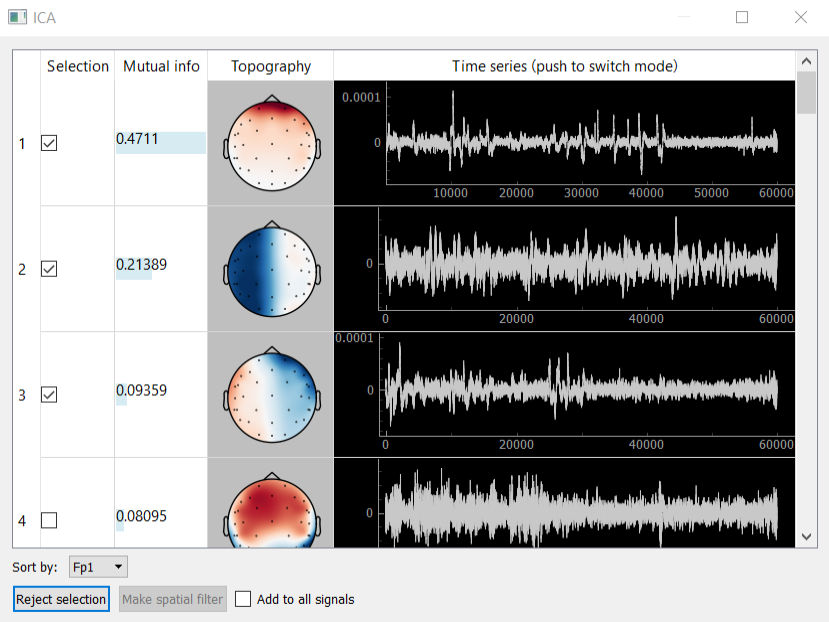
\includegraphics[width=0.7\linewidth]{ica}
\caption{Example of using NFBLab to remove eye artifacts with ICA before running the main part of the experiment \cite{Smetanin2016}}\label{fig:ica}
\end{figure}

NFBLab has a feature of designing eye artifact filters. Before the main part of experiment it is possible to record a baseline section and apply ICA on it. Then, it is possible to sort components by the mutual information with a certain channel. In our case, these channels would be Fp1 and Fp2, because they record eye blinks with the largest amplitude). After selecting the components, that we want to exclude from the data, for the selected signals a spatial filter removing the selected ICA components will be created.

\subsection{Data Analysis}
\label{sec:Methods:Data{} Analysis}

Here we summarize various data analysis methods that were explicitly implemented in the code. The methods that were presented in the software packages are set up with references. At the end of the section, the data processing procedures that were applied in the study are summarized. 

\subsubsection{Z-score}
\label{sec:Methods:Data Analysis:Z-score}

\begin{figure}[H]
\centering
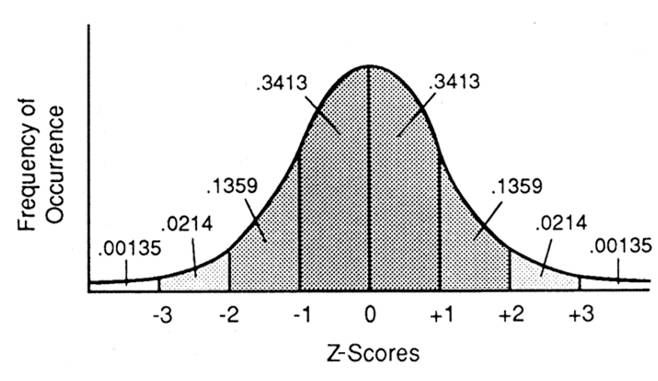
\includegraphics[width=0.7\linewidth]{z-scores.jpg}
\caption{Z-score on a normal distribution and corresponding $p-values$}\label{fig:z-scores.jpg}
\end{figure}

\textit{Z-scores (z-values, normal scores, standard scores standardized variables)} is the standard deviations $\sigma$ signed number by which a data point value $x$ is above the measured mean value $E[X]$ (Eq.~\ref{eq:zscore}). This statistic is frequently used to compare a data point to a standard normal variable, so the $p-value$ can be calculated from it easily (Fig. \ref{fig:z-scores.jpg}). 

\begin{equation} \label{eq:zscore}
Z = \frac{x - E[x]}{\sigma}
\end{equation}

\subsubsection{Common Spatial Pattern}
\label{sec:Methods:Data Analysis:Common Spatial Pattern}

The common spatial pattern (CSP) technique maximizes the difference between two windows $X_{1}$ and $X_{2}$ of the multivariate signal for separating into additive subcomponents (Eq. 1). If $X_{i}$ is a matrix $n_{i}$ by $t_{i}$, where $n_{i}$ – number of channel and $t_{i}$ – number of samples, such a problem can be solved by computing the two covariance matrices (Eq. 2) and the subsequent spectral decomposition of these two matrices (Eq. 3).

The $CSP(X1, X2)$ function used in the following sections gets two windows of the multivariate signal as arguments and returns an eigenvalue corresponding to the analyzed component that should be used in the next statistical test.

\begin{equation}
w = \argmax_{w}{\frac{\left \| wX_{1} \right \|}{\left \| wX_{2} \right \|}}
\end{equation}
\begin{equation}
C_{i} = \frac{X_{i}X^{T}_{i}}{t_{i}}
\end{equation}

\begin{equation}
C^{-1}_{2}C_{1} = PDP^{-1}
\end{equation}


\subsubsection{Tikhonov Regularization}
\label{sec:Methods:Data Analysis:Tikhonov Regularization}

\textit{The Tikhonov regularization}, or sometimes $L_2$ regularization \cite{Ng2004}, that is called after \textit{Andrey Tikhonov}, a Soviet and Russian mathematician and geophysicist, is the most commonly used method of regularization of ill-posed problems $Ax = u$. 

The basic idea is to find an approximate solution of the equation $Ax = u$ in the form $x_{\delta} = R(u_{\delta}\alpha)$, where $R(u_{\delta}\alpha)$ is the regularizing operator, $\alpha$ – hyperparameter ($\alpha > 0$). When $u_{\delta} \rightarrow u_{T}$, while $\delta \rightarrow 0$, the approximate solution $x_{\delta} \rightarrow x_{T}$ of the equation $Ax = u_{T}$.

In a general form, which was applied in our algorythm, Tikhonov's regularization can be formulated in the following form: 

\begin{equation}
x' = x_0 + (A^{T}PA + Q)^{-1}(A^{T}P(b-Ax_{0})),
\end{equation}

where $x'$ is the optimal solution, $x_0$ is the mathematical expectation of $x$, $P$ is the covariance matrix, and $Q$ is the inverted covariance matrix $x$ \cite{Tikhonov1963}.

In our case the Tikhonov regularization is applied to eigendecomposition $C^{-1}_{2}C_{1} = PDP^{-1}$ in an ill-posed CSP case.

\subsubsection{Nonparametric Statistical Testing Of EEG Data}
\label{sec:Methods:Data Analysis:Nonparametric Statistical Testing Of EEG Data}

\begin{figure}[H]
\centering
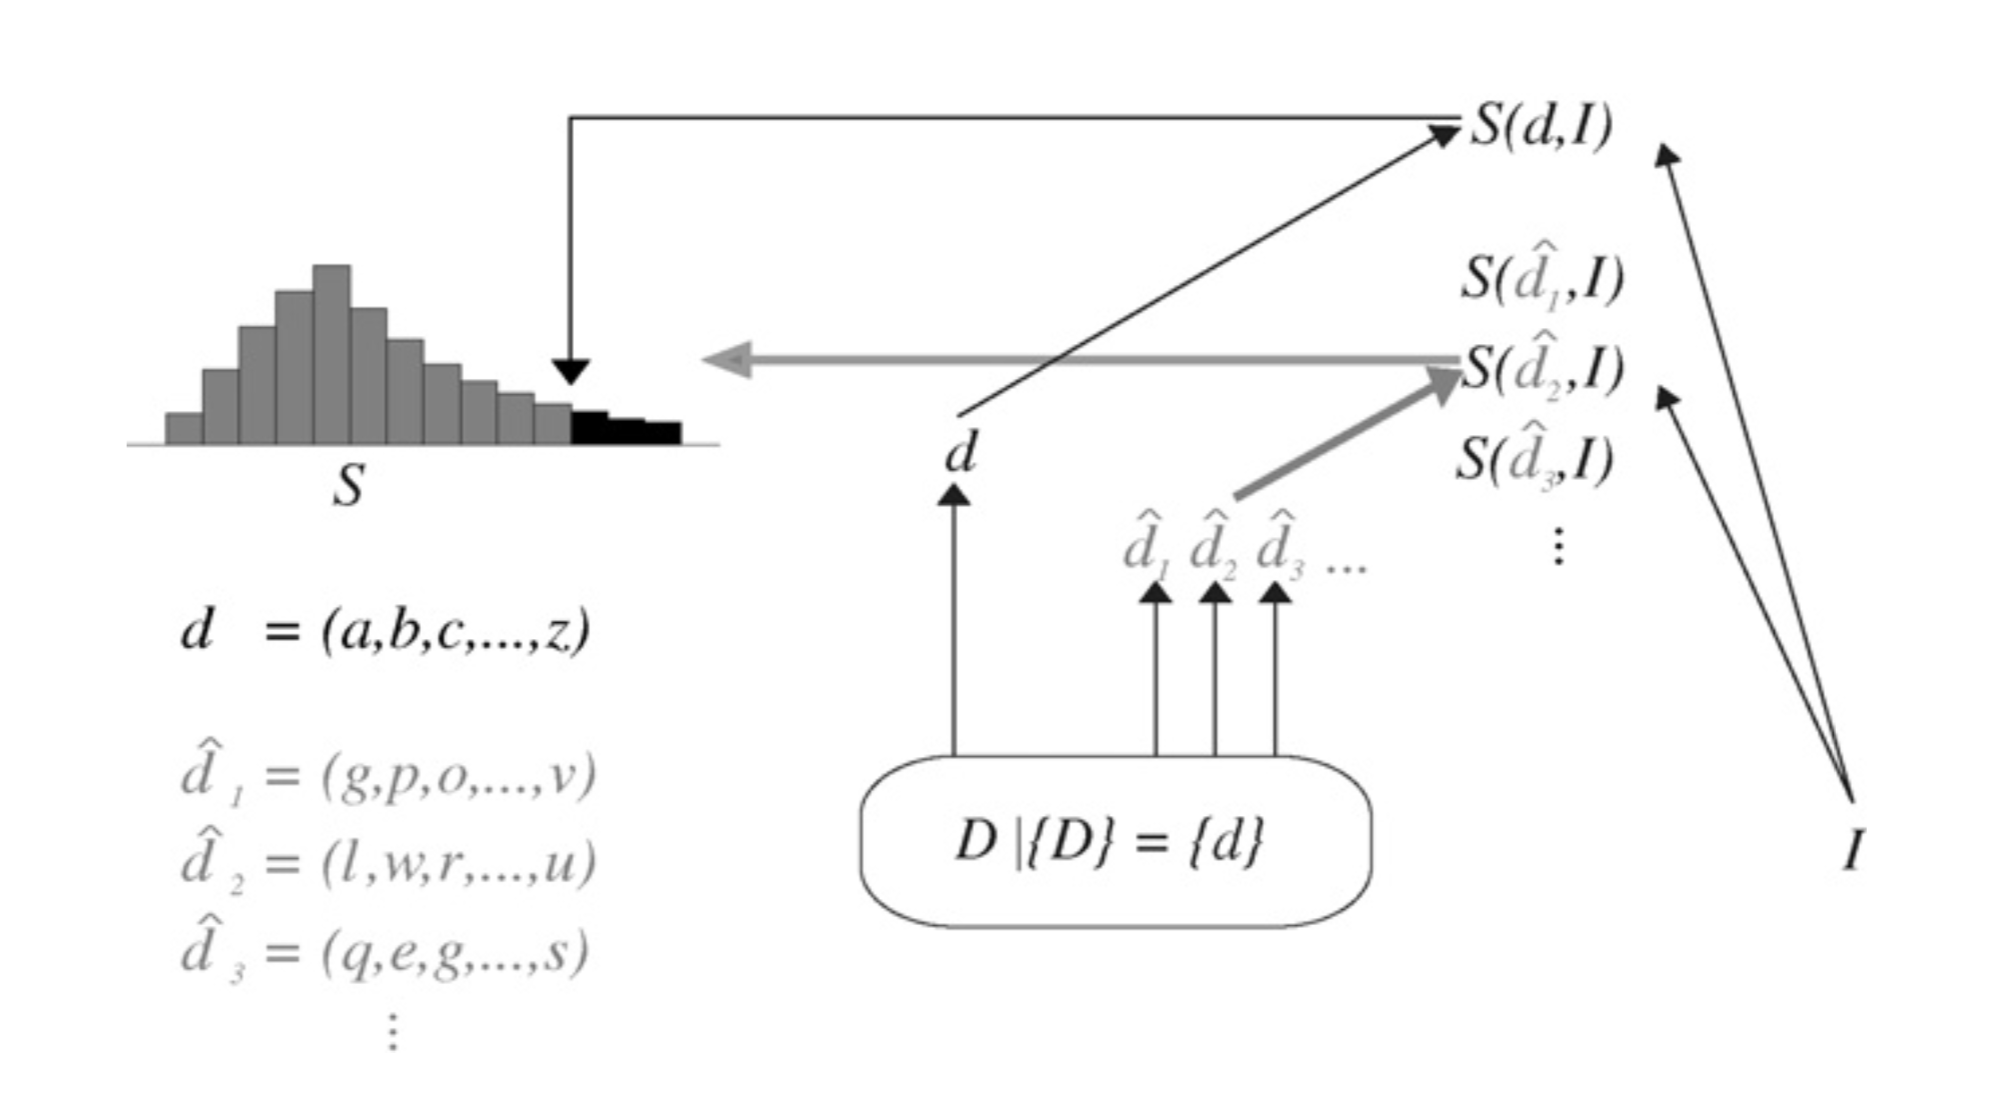
\includegraphics[width=0.7\linewidth]{nps}
\caption{Comparison of the statistic for the real signal with the resulting zero distribution generated by permutations \cite{Maris2007}}\label{fig:nps}
\end{figure}

In our study we tested the null hypothesis $H_0: F(D_r| I=1) =  F(D_r|I=2)$, where $D_r (r = 1, . . . , n)$ are the protocols to which the data was divided for two different conditions. 

The following statistics function was used: $S(d_r, I) = CSP(X_1, X_2)$, where $d_r$ is the observed signal; $X_1$ is the signal window for the first condition, $X_2$ is the signal window for the second condition.

The zero distribution was calculated as follows: $S(d_r, I) ~ F(S(D, I)|{D} = {d})$, where ${d}$ is the permuted signal \cite{Maris2007}. 

\subsubsection{False Discovery Rate Correction}
\label{sec:Methods:Data Analysis:False Discovery Rate Correction}

Assume that $N$ hypotheses $H_1, H_2 ... H_n$ were tested. Resulting $p-value$ values are $p_1, p_2, ... p_n$ respectivly. The parameter $q$, the maximum number of falsely rejected null hypotheses, is defined. Then the $p-value$ are sorted in ascending order: $p^*_1 \leqslant p^*_2 \leqslant ... , \leqslant p^*_n$. $p^*_i$corresponds to $H^*_i$.

\begin{equation}
p(i) \leqslant \frac{iq}{N}
\end{equation}

According to Eq. 5, $p^*_i$ is chosen, for which $H^*_1, ... , H^*_{i-1}$ is rejected. 

\begin{equation}
q(i) \leqslant \frac{p_N}{i}
\end{equation}

The value of $q$ can be calculated not for the entire p-value set, but for each $p^*_i$ separately (Eq. 6), which was applied in our algorithm \cite{Benjamini1995}.

Later, the authors proposed a modification of the correction for those cases in which independence can not be proved \cite{Benjamini2001}. In our case, the significance of the difference between the eigenvalues and the zeroth distribution is tested. They characterize linearly independent eigenvectors, and therefore independence is proved for them.

\subsection{Experimental Design}
\label{sec:Methods:Experimental Design}

For each participant we recorded the electroencephalography data for mock and real feedback conditions at 500 Hz sampling rate with NVX 132 encephalograph.

The neurofeedback method was used in the experiment. It was implemented with the help of NFBLab software \cite{Smetanin2016}. Using this method, we decided to train the occipital alpha wave of the subject, as it was the easiest one to evoke. Moreover, the artificial training of this wave for healthy people does not lead to any disorders. The aim of the study was to reveal the correlates of effective learning in the frontal beta-rhythm associated with the performance on the tasks.

Before the main part of the experiment, a 1 minute closed eyes and open eyes trails were recorded. They were meant to collect data on eye movements to adjust the filter that removes eye artifacts during the experiment. After the filter was set up, the main part of the experiment began. The subjects were trained either with real feedback of their alpha waves discrete power extracted from the P4 electrode or with mock-feedback. However, subjects did not know that mock trails would be presented to them. During the training they were instructed to sit as still as possible and focus on the visual feedback in the form of a game in which a spacecraft was flying from the earth to the space. While the subjects were performing the task assigned to them, their encephalogram was processed in real time. Two signals were calculated based on the encephalogram obtained from P4 electrode. 

The first signal was an alpha envelope. A signal was filtered in the alpha band using a Butterworth filter. Then, the absolute value of signal was taken. Finally, the signal was exponentially smoothed. A signal in such form represents an alpha power estimate. 

The second signal was 95 percent quantile of the alpha envelope. In this study, it is essential for neurofeedback demonstrate and is the center of this paradigm. Both NVX132 and NFBLab exchange data by means of so called chunks, small picies of EEG data, that are send or recieved by machine or software each few milliseconds. While NVX132 and NFBLab either send or recieve chunks, <<Vapour Track>> is only able to recive them. Each data chunk that would be recieved by <<Vapour Track>> from the NFBLab, represents the power estimate, or, in other words, the value of the first signal at a given time. When the recording begins, one value is added to the time buffer with the first chunk. When a new chunk arrives, the $i-th$ power estimate value is written to the buffer. The buffer can store information brought by $n$ chunks within 10 seconds in $n$ cell, shifting $i-th$ value to the end of the buffer by one cell. When 10 seconds pass, the last value $n$ leaves the buffer, leaving an empty cell at its beginning. Thus, the second signal is the 95 percent quantile value of the alpha power estimate. Based on the 10 second information, a 95 percent quantile is computed, which is the second signal and is updated every time a new chunk arrives.

Each time the value of the first signal was crossing the value of the second signal, the spacecraft would fly upwards, thus being a discrete reinforcement. Then there was a three-second period of refractoriness, when the spacecraft did not move. Such a time interval was chosen by taking into account the average length of the alpha spindle \cite{Bazanova2014}. The time intervals between individual reinforcements were also stored in a separate buffer. Random intervals were extracted from this buffer when a false feedback was displayed. It was done so that the reinforcement dynamics in the subject did not differ much from the real to mock trails. Each time the reinforcement was presented, the EEG data was stamped using a photosensor in order to calculate the ERP.

Each session consisted of 4 experimental trials 7 minutes long each. Real trail was followed by mock trail and then such sequence was repeated on more time. Subjects were given time to rest between the trails. When the data was recorded, four different processing procedures were applied to them. Note that in this paradigm we did not aim at training alpha and find the difference in it between real and mock trails but rather attempted to catch the low-level difference between the consistent and inconsistent feedback as it is perceived by the brain.

The data were then filtered with a band-pass finite impulse response filter in 30 different frequency bands from 1-30 Hz range with 2 Hz bandwidth. The the data was cut to small pieces. The beginning of the piece was considered to be when the reinforcement was presented. The end of the stimuli was 1000 ms later. The data pieces from the two conditions (real and mock feedback) were contrasted using the common spatial pattern procedure. Common spatial pattern is a mathematical technique that separates a multivariate signal into subcomponents with maximum differences in variance between two windows \cite{Koles1990}. It is used in the field of digital signal processing to compare two types of data and to stress the difference between them.

In order to establish the significance of the observed differences we performed non-parametric randomization test to obtain the $p-values$ of null hypothesis of no significant changes between the real and mock feedback conditions \cite{Maris2007}. Next, a correction for the number of false detection rate was applied to the obtained $p-value$ \cite{Benjamini2001}.

To test the effectiveness of the mathematical algorithm described above, we first decided to test the quality of the algorithm on conditions in which the activation is obviously distinguishable: on the eyes-open condition, when the occipital alpha-rhythm is absent, and on the eyes-closed condition, when the alpha rhythm is present.


\newpage
\section{Results}
\label{sec:Results}  

Firstly, our algorithm managed to tell the eyes-open condition from the eyes-closed condition. We found statistically significant components in the alpha band, with occipital localization which definitely corresponds to visual cortex.

Secondly, we applied our algorithm to data received from four experimental electroencephalographic recordings. Although we expected to find the activation in the beta band, with frontal localization which may correspond to the anterior cingulate cortex, which activity contrasts with the real feedback and mock feedback conditions, no statistically significant differences were found.

\newpage
\section{Conclusions}
\label{sec:Conclusions} 

Since we did not find any activation localized in the frontal regions that could have been consistent to the previous studies, it is important to continue the research. In the further study, learning conditions in the neural feedback paradigm should be improved and the optimal design for the selection of the frontal beta-rhythm should be found.

We’re still not certain if the areas related to effective learning may be used to improve the technique of neural feedback, having the ability to monitor therapy in this paradigm and with the accuracy to establish whether this method is suitable for patients.

\newpage
\section*{Acknowledgements}
\label{sec:Acknowledgements}
\addcontentsline{toc}{section}{Acknowledgements}

I would like to express my gratitude to my advisor professor Alexey E. Ossadtchi, PhD, for the continuous support of my undergraduate thesis study and research, for suggesting me the hard, but incredibly interesting research problem, for his comments, suggestions and immense knowledge.

I would also like to give my thanks to Nikolai M. Smetanin, MSc, for his help in programming, math and physics, and for moral support in difficult times. 

I really appreciate the help provided by Alina Heiremans, checking the literacy of my English text.

\newpage
\section*{Appendices}
\label{sec:Appendices}
\addcontentsline{toc}{section}{Appendices}

\newpage
\bibliographystyle{apa}
\bibliography{/Users/wassilyminkow/Scripts/LaTeX/library.bib}
\end{document}